\chapter{Laços de Repetição}
\label{cap:lacos}

Frequentemente precisamos construir algoritmos que repitam operações. Esta repetição pode ter uma quantidade determinada de vezes: 0 a 10, por exemplo. Pode ocorrer de um valor menor até outro maior: -5 até 5, por exemplo. Pode ir de um valor maior até outro menor: 100 até 25, por exemplo. As repetições podem ocorrer nos mais diversos cenários e modos.

Para trabalhar com repetição, é preciso compreender o básico das técnicas de controle de repetição, ou laços de repetição. Nesta sessão, vamos conhecer as principais técnicas para controle de repetição.

\section{Laço While}
A palavra while pode ser traduzida para enquanto.

\emph{-> -> A instrução while executa um laço do tipo “enquanto-faça”   <- <-}

Nesta técnica repetimos um conjunto de instruções enquanto uma determinada condição for verdadeira. Utilizamos while quando queremos que um determinado bloco de código seja executado ENQUANTO uma determinada condição seja VERDADEIRA. No momento em que a condição for FALSA, o bloco de código deixa de ser repetido.

O fluxograma na Figura~\ref{fig:lacosimples} a seguir demonstra graficamente este tipo de repetição.

\begin{figure}[h]
  \begin{center}
    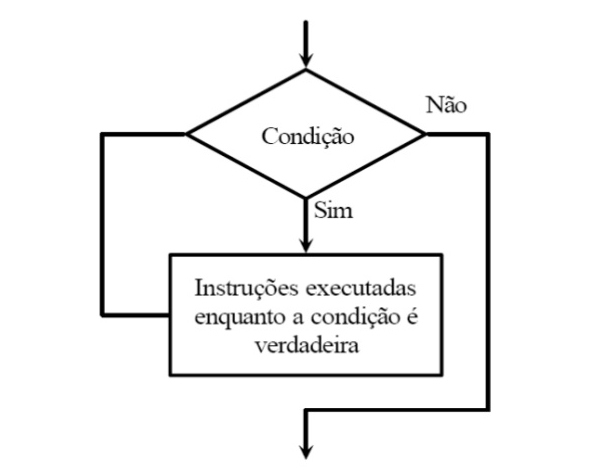
\includegraphics[width=0.5\textwidth]{img/laco.png}
    \caption{Fluxograma demonstrando um laço de repetição.}
    \label{fig:lacosimples}
  \end{center}
\end{figure}


Para demonstrar o uso desta estrutura de laço, apresentamos 3 exemplos simples. As soluções dos problemas serão demonstradas usando representação gráfica de fluxograma;  representação em Pseudocódigo; com Javascript e com Octave. 

\subsubsection{Problema 1}
Escreva um algoritmo/programa para \emph{mostrar na tela os números de 1 até 10, usando repetição.}

\subsubsection{Fluxograma}
A Figura~\ref{fig:problema1} mostra um algoritmo, que resolve este problema, representado em fluxograma. 

Para resolver o problema criamos uma variável (i) com valor inicial 1; no losango representamos a verificação do laço, onde o algoritmo testa se a variávei i ainda é menor ou igual a 10; se i ainda é menor/igual a 10, o programa mostra o valor de i e faz com que a variável i receba o valor de i mais 1 (chamamos isso de incremento de variável). Caso o teste de i seja maior que 10, então o fluxo é desviado para o fim do programa.

\begin{figure}[h]
  \begin{center}
    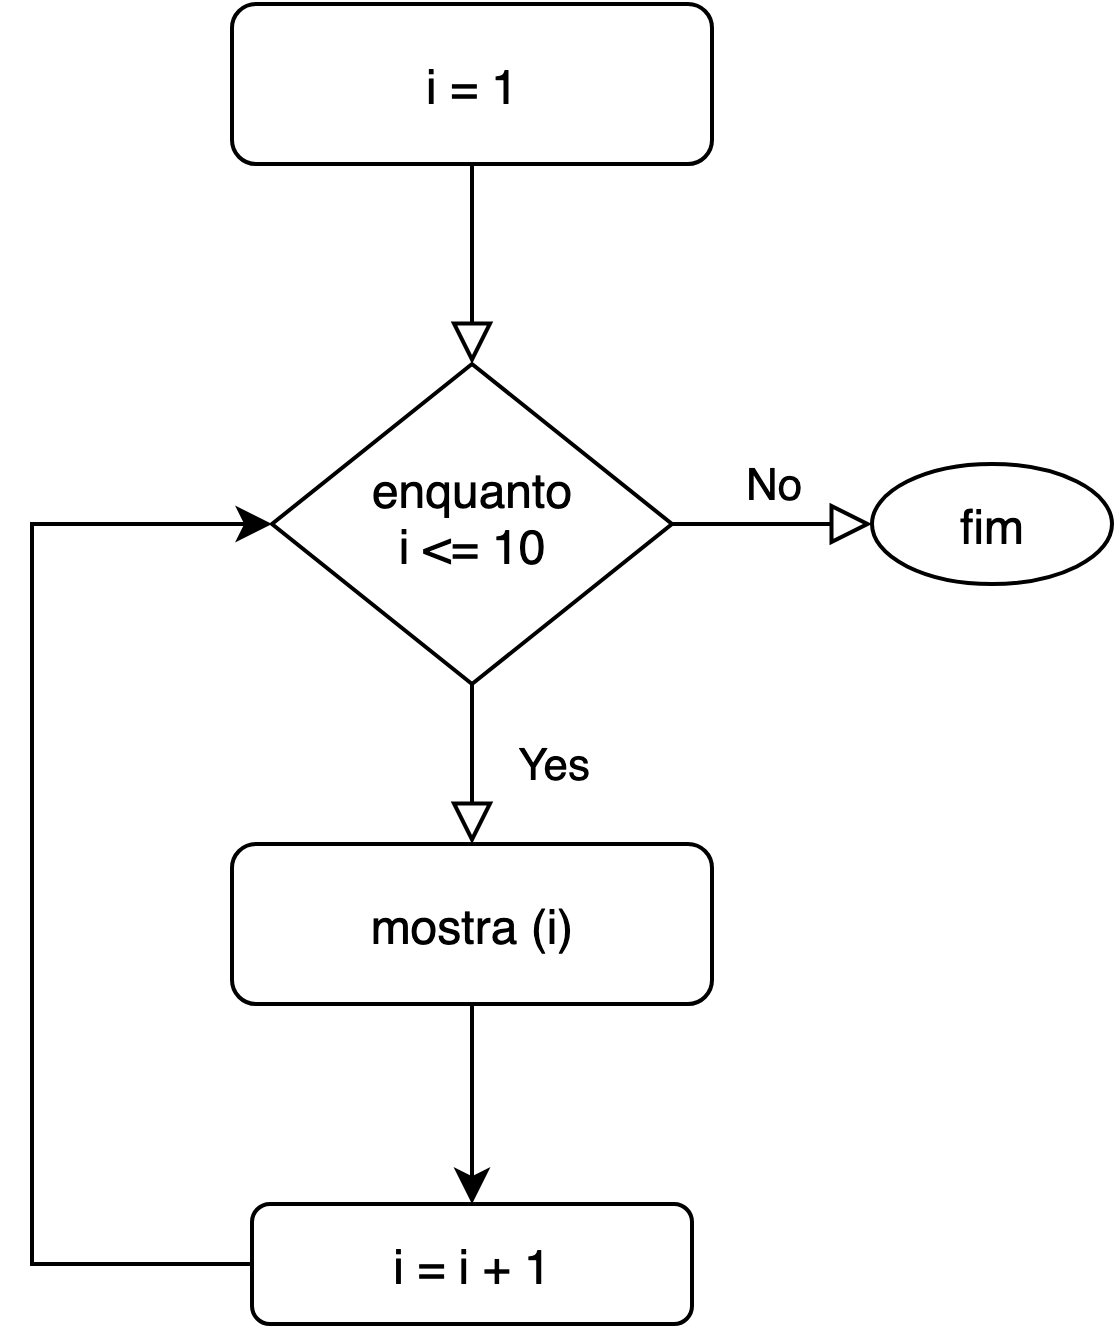
\includegraphics[width=0.5\linewidth]{img/problema1.png}
    \caption{Fluxograma representando a solução do problema 1.}
    \label{fig:problema1}
  \end{center}
\end{figure}

\subsubsection{Pseudocódigo}
\begin{verbatim}
Início
var i := 1
enquanto i <= 10, repita:
          mostra i
          i = i + 1
fim-enquanto

Fim
\end{verbatim}


\subsubsection{Javascript}
\subsubsection{Octave}



Javascript
var i = 1;
while( i <= 10){
  print(i);
  i = i + 1;
}

Octave
clear
i = 1
while (i <= 10)
  printf(" %d ",i)
  i++
endwhile

Observe que a estrutura de uso da instrução while é semelhante nas linguagens JavaScript e Octave. No código em octave, a instrução i++ é equivalente a instrução i = i+1 
Escolha uma das linguagens e execute o trecho observando o teste que ocorre dentro do parênteses. Observe o resultado se tirarmos o sinal de “=” o laço repete de 1 até 9.
